\documentclass[../main.tex]{subfiles}
%%\documentclass[14pt,a4paper,twoside]{extarticle}	% Размер основного шрифта и формата листа
%\usepackage{xltxtra,xunicode,polyglossia}						% Используется для вывода логотипа XeLaTeX
%\newfontfamily\russianfont{Liberation Serif}
%\usepackage{standalone}
%\usepackage{tikz}
%\setdefaultlanguage{russian}				% Основной язык текста
%\setotherlanguage{english}					% Дополнительный язык текста
%\linespread{1}							% Межстрочный интервал выбран полуторным
%\usepackage[left=2.5cm,right=1.5cm,vmargin=2.5cm]{geometry} % Отступы по краям листа
%
%\usepackage{xcolor,hyperref}
%\definecolor{linkcolor}{HTML}{359B08} % цвет ссылок
%\definecolor{urlcolor}{HTML}{799B03} % цвет гиперссылок
%\hypersetup{pdfstartview=FitH,  linkcolor=linkcolor,urlcolor=urlcolor, colorlinks=true}
%
%\usepackage{verbatim,indentfirst,cite,enumerate,float,amsmath,amssymb,amsthm,amsfonts}
%\usepackage{graphicx,fontspec,subfigure}

%\usepackage{xltxtra,xunicode,polyglossia}						% Используется для вывода логотипа XeLaTeX
%\newfontfamily\russianfont{Liberation Serif}
%\usepackage{subfiles}
%\setdefaultlanguage{russian}				% Основной язык текста
%\setotherlanguage{english}					% Дополнительный язык текста
%\linespread{1}							% Межстрочный интервал выбран полуторным
%\usepackage[left=2.5cm,right=1.5cm,vmargin=2.5cm]{geometry} % Отступы по краям листа
%
%
%\usepackage{xcolor,hyperref}
%\definecolor{linkcolor}{HTML}{359B08} % цвет ссылок
%\definecolor{urlcolor}{HTML}{799B03} % цвет гиперссылок
%\hypersetup{pdfstartview=FitH,  linkcolor=linkcolor,urlcolor=urlcolor, colorlinks=true}
%
%\usepackage{verbatim,indentfirst,cite,enumerate,float,amsmath,amssymb,amsthm,amsfonts}
%\usepackage{graphicx,fontspec,subfigure}


\begin{document}
%	\pagestyle{empty} %  выключаенм нумерацию
%\setcounter{page}{3}% Нумерация начинается с третьей страницы
%\renewcommand{\contentsname}{\center{Содержание}}
%\tableofcontents

\newpage
\begin{center}
%	\addcontentsline{toc}{section}{Опыт 6. Сложение угловых скоростей}
	\subsection*{Сложение угловых скоростей}
\end{center}

\begin{figure}[H] 
	\centering 	
	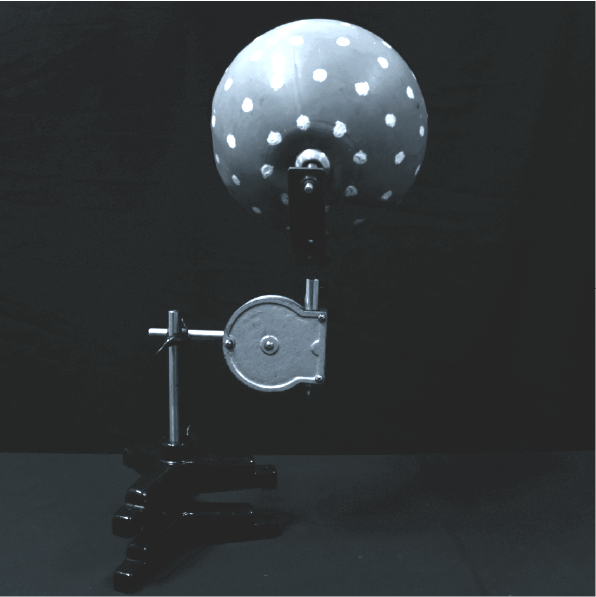
\includegraphics[width=0.6\linewidth]{angular-1.png}
	\caption{Демонстрация сложения угловых скоростей на центробежной машине}
	\label{angular-1}
\end{figure}

\subsection*{\underline{Оборудование:}}

\begin{enumerate}
	\item Шар диаметром 35 см, покрытый по линиям широт рядами пятен белого цвета диаметром 1 см.
	\item Вращающийся держатель.
	\item Машина с червячным механизмом.
\end{enumerate}

\subsection*{\underline{Основные определения:}}

Угловая скорость — величина, характеризующая быстроту вращения твердого тела. 
При равномерном вращении тела вокруг неподвижной оси его угловая скорость численно равна приращению угла поворота $ \varphi $ за промежуток времени $ \Delta t $
$$ \omega = \Delta \varphi/ \Delta t. $$
 
В общем случае угловая скорость численно равна отношению элементарного угла поворота $d\varphi $ 
к соответствующему элементарному промежутку времени $ dt $, то есть $$ \omega = d\varphi/dt. $$ 

Таким образом,
\begin{flushleft}
	\textit{вектор угловой скорости} \textbf{ω} \textit{численно равен величине угловой скорости, лежит на оси вращения, и направление его связано с направлением вращения согласно правилу буравчика}.
\end{flushleft}

Поскольку угловая скорость — вектор, то приращение ее также вектор и, следовательно, вектором является угловое ускорение:
$$ \textbf{ε} = \frac{d\textbf{ω}}{dt}.$$

Между векторами угловой и линейной скоростей для каждой материально точки твердого тела существует связь.
\begin{flushleft}
	\textit{Вектор линейной скорости точки при вращательном движении равен векторному произведению вектора угловой скорости на радиус-вектор точки}
\end{flushleft}
$$ \textbf{v} = \textbf{ω}\times \textbf{r}. $$

\subsection*{\underline{Краткое описание:}}

Шар закрепляется в специальном держателе, в котором он может вращаться вокруг наклонной оси, а вместе с держателем — вокруг вертикальной оси при помощи червячной машины.
Таким образом вращать шар можно либо вокруг наклонной оси, либо вокруг вертикальной оси, либо вокруг обеих осей одновременно.

При быстром вращении шара вокруг наклонной оси пятна на его поверхности сливаются и образуют параллельные ряды (рис.\ref{angular-2},\textit{а}), перпендикулярные к оси вращения.
Направление оси вращения шара совпадает с направлением угловой скорости вращения $ \textbf{ω}_{1} $.

\begin{figure} 	
	\centering 	
	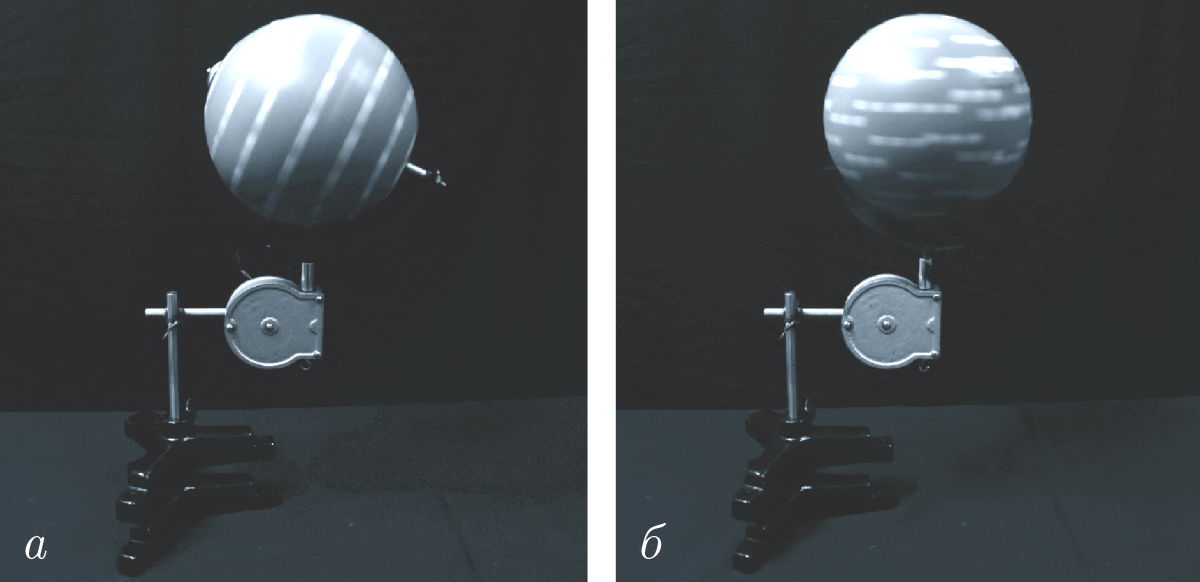
\includegraphics[width=0.85\linewidth]{angular-2.png}
	\caption{\textit{а} — вращение шара только вокруг наклонной (собственной) оси; \textit{б} — вращение шара только вокруг вертикальной оси}
	\label{angular-2}
\end{figure}

При вращении шара только вокруг вертикальной оси пятна сливаются в линии (рис.\ref{angular-2},\textit{б}), которые лежат в горизонтальных плоскостях, перпендикулярных оси вращения держателя, вдоль которой направлен вектор $ \textbf{ω}_{2} $.

В ходе эксперимента обнаруживаем, что при одновременном вращении шара вокруг собственной оси и вокруг оси вращения держателя светлые пятна на его поверхности перемещаются таким образом, будто вращаются вокруг новой движущейся оси - мгновенной оси вращения твердого тела.

\subsection*{\underline{Теория:}}

Когда материальная точка участвует в нескольких независимых движениях, то для перемещений, скоростей и ускорений справедливы правила векторного сложения, при этом результирующее перемещение равно векторной сумме отдельных независимых перемещений.

\begin{figure}[H] 	
	\centering 	
	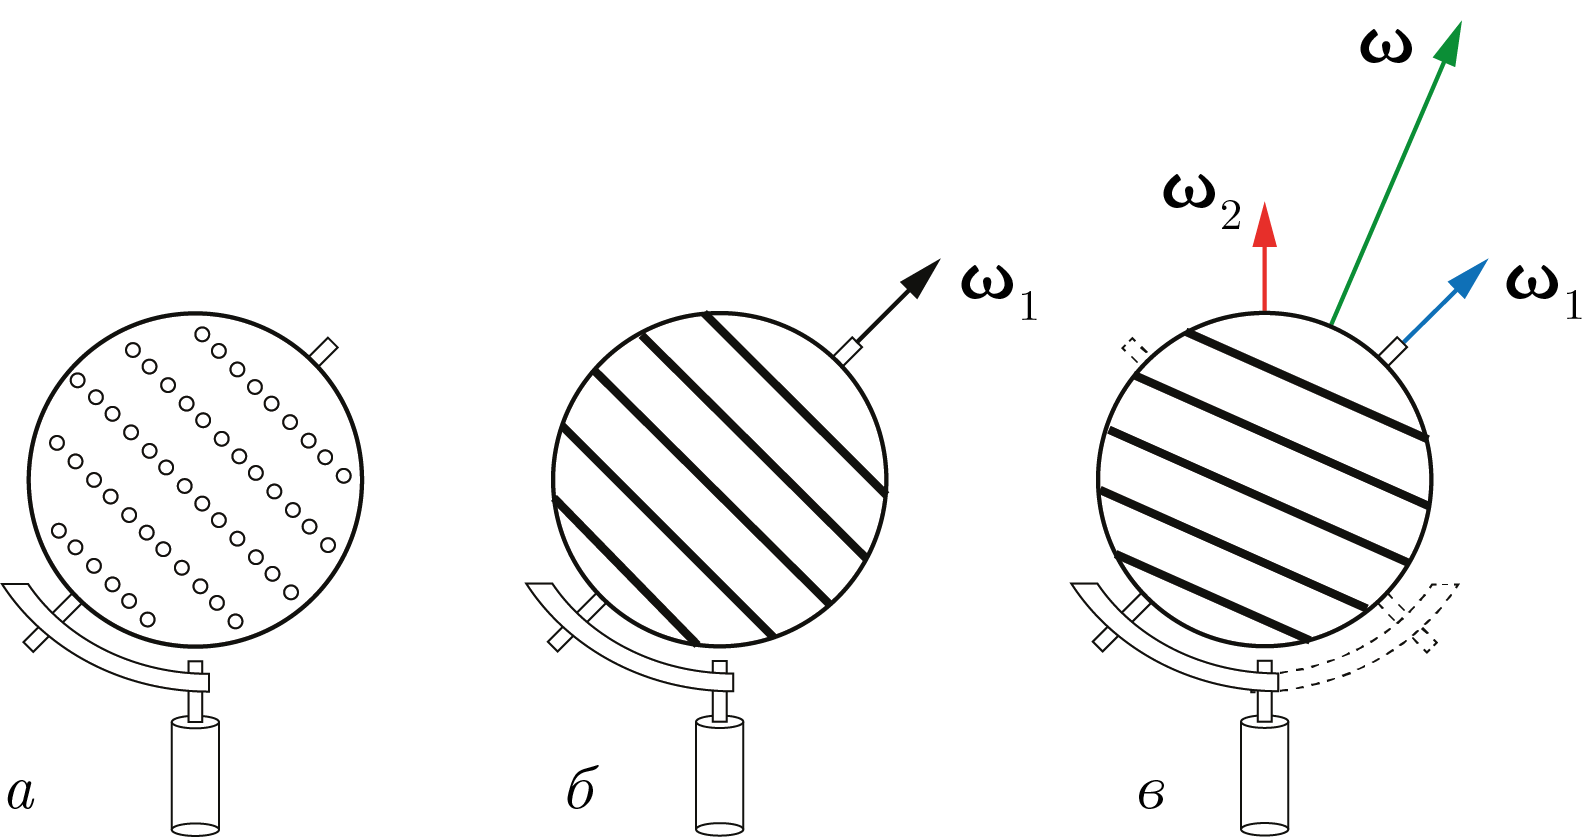
\includegraphics[width=0.8\linewidth]{angular-3.png}
	\caption{\textit{а} — схематичное изображение шара на вращающемся стержне (без вращения); \textit{б} — вектор угловой скорости при вращении шара только вокруг собственной (наклонной) оси; \textit{в} — сложение угловых скоростей при одновременном вращении шара вокруг собственной и вертикальной осей}
	\label{angular-3}
\end{figure}

В классической механике закон сложения скоростей Галилея позволяет определить результирующую скорость материальной точки относительно неподвижной системы отсчета, которая движется во вращающейся системе отсчета. Для точки на поверхности шара, движущейся одновременно вокруг вертикальной оси со скоростью $\textbf{v}_1$ и наклонной оси со скоростью $\textbf{v}_2$, результирующую линейную скорость $\textbf{v}$ можно представить в виде:

\begin{equation}\label{angular-eq1}
\textbf{v} = \textbf{v}_1 + \textbf{v}_2.
\end{equation}

Используя известную связь между линейной и угловой скоростями, можно получить следующее выражение:
\begin{equation}\label{angular-eq2}
\textbf{v} = \textbf{ω}_1 \times \textbf{r} + \textbf{ω}_2 \times \textbf{r} = (\textbf{ω}_1 + \textbf{ω}_2) \times \textbf{r} ,
\end{equation}
где через \textbf{r} обозначен радиус-вектор, направленный из центра шара в рассматриваемую точку на его поверхности.

Следовательно, при одновременном вращении шара и держателя, результирующая угловая скорость \textbf{ω} также будет представлять собой векторную сумму $ \textbf{ω}_1 $ и $ \textbf{ω}_2 $, и иметь направление, показанное на рис.\ref{angular-3},\textit{в}.
Это направление легко определить опытным путем так как кружки, расположенные вблизи мгновенной оси (вдоль вектора \textbf{ω}), не сливаются в линии.

Таким образом, при одновременном вращении шара вокруг собственной оси и вокруг оси вращения держателя вектор результирующей угловой скорости, а, следовательно, и мгновенная ось вращения также поворачиваются вокруг вертикальной оси держателя. Величина угловой скорости вращения шара относительно мгновенной оси вращения равна векторной сумме угловой скорости вращения шара вокруг своей оси и угловой скорости поворота оси шара $ \textbf{ω} = \textbf{ω}_1 + \textbf{ω}_2 $.

\end{document}